\documentclass[a4paper,12pt]{article}
\usepackage[utf8x]{inputenc} %fac
%\usepackage[utf8]{inputenc} %fac

%\usepackage[square,sort,comma]{natbib}
%\usepackage{chapterbib}

\usepackage[francais]{babel} %FR
\usepackage[T1]{fontenc}
\usepackage{fancyhdr}
\usepackage{multicol}

\usepackage[pdftex]{graphicx} % img
%\usepackage{wrapfig} %fac
\usepackage{float}

%\usepackage{algpseudocode} %fac
\usepackage[hidelinks]{hyperref} %fac

\usepackage[top=3.5cm, bottom=3.5cm, left=3cm, right=3cm]{geometry} %Réduire les marges

% \usepackage{showkeys}
% \usepackage{showlabels}
\usepackage{nameref}

\usepackage{color}
\usepackage{listings}

% Style Page
\pagestyle{fancy} % entêtes

\setlength{\headheight}{15pt}
\lhead{ \leftmark }
\rhead{ %\rightmark 
}

\sloppy % ne pas faire déborder les lignes dans la marge

%\setcounter{tocdepth}{1} %hideallsubsections


 
% Definition de couleur supplementaire
\definecolor{colString}{rgb}{0.6,0.1,0.1}
 
% Definition du langage
\lstdefinelanguage{LangageConsole}{%
    morekeywords={%
        ligne% mot-clé ``ligne''
    }
}
 
% Definition du style
\lstdefinestyle{styleLangage}{%
    language        = LangageConsole,%
    basicstyle      = \footnotesize\ttfamily\color{white},% ecriture standard
    identifierstyle = \color{white},%
    commentstyle    = \color{green},%
    keywordstyle    = \color{blue},%
    stringstyle     = \color{colString},%
    extendedchars   = true,% permet d'avoir des accents dans le code
    tabsize         = 2,%
    showspaces      = false,%
    showstringspaces = false,%
%     numbers=left,%
    numberstyle=\tiny\ttfamily\color{black},%
    breaklines=true,%
    breakautoindent=true,%
        backgroundcolor=\color{black},%
}
 
\lstset{%
    style = styleLangage%
}

\begin{document}
  \begin{titlepage}
   \def\titletype{Manuel de l’utilisateur}
   %%%%%%%%%%%%%%%%%%%%%%%%%%%%%%%%%%%%%%%%%
% University Assignment Title Page
% LaTeX Template
%
% This template has been downloaded from:
% http://www.latextemplates.com
%
% Original author:
% WikiBooks (http://en.wikibooks.org/wiki/LaTeX/Title_Creation)
%
% Instructions for using this template:
% This title page is presently capable of being compiled as is. This is not
% useful for including it in another document. To do this, you have two options:
%
% 1) Copy/paste everything between \begin{document} and \end{document}
% starting at \begin{titlepage} and paste this into another LaTeX file where you
% want your title page.
% OR
% 2) Remove everything outside the \begin{titlepage} and \end{titlepage} and
% move this file to the same directory as the LaTeX file you wish to add it to.
% Then add \input{./title_page_1.tex} to your LaTeX file where you want your
% title page.
%
%%%%%%%%%%%%%%%%%%%%%%%%%%%%%%%%%%%%%%%%%

%----------------------------------------------------------------------------------------
%       PACKAGES AND OTHER DOCUMENT CONFIGURATIONS
%----------------------------------------------------------------------------------------

\begin{titlepage}

\newcommand{\HRule}{\rule{\linewidth}{0.5mm}} % Defines a new command for the horizontal lines, change thickness here

\center % Center everything on the page

%----------------------------------------------------------------------------------------
%       HEADING SECTIONS
%----------------------------------------------------------------------------------------

\textsc{\LARGE Pierre and Marie Curie University}\\[1.5cm] % Name of your university/college
\textsc{\Large \titletype}\\[0.5cm] % Major heading such as course name
%\textsc{\large PIAD de Master1 d’Informatique en Intelligence Artificielle et Décision}\\[0.5cm] % Minor heading such as course title

%----------------------------------------------------------------------------------------
%       TITLE SECTION
%----------------------------------------------------------------------------------------

\HRule \\[0.4cm]
{ \huge \bfseries \majortitle}\\[0.4cm] % Title of your document
\HRule \\[1.5cm]


%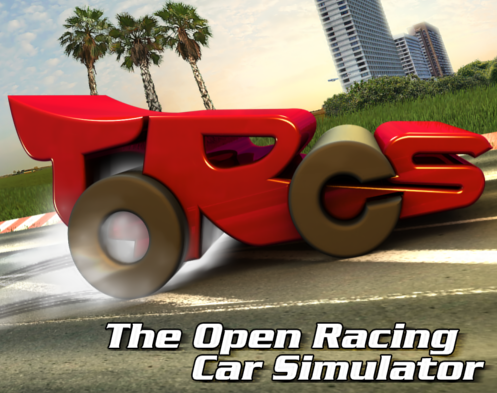
\includegraphics[height=60mm]{images/torcs.png}\\[1cm]


%----------------------------------------------------------------------------------------
%       AUTHOR SECTION
%----------------------------------------------------------------------------------------

\begin{minipage}{0.4\textwidth}
\begin{flushleft} \large
\emph{Author:}\\
Matthieu \textsc{Zimmer} % Your name
\end{flushleft}
\end{minipage}
~
\begin{minipage}{0.4\textwidth}
\begin{flushright} \large
\emph{Supervisors:} \\
Paolo \textsc{Viappiani}\\ % Supervisor's Name
Paul \textsc{Weng}\\ % Supervisor's Name
\end{flushright}
\end{minipage}\\[1cm]

\vfill

%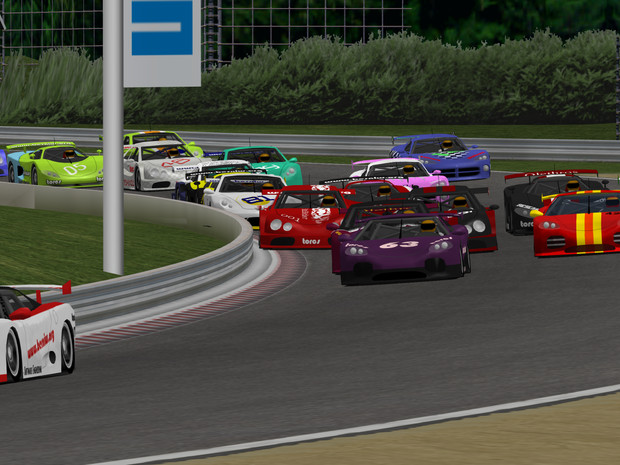
\includegraphics[height=70mm]{images/torcs.jpg}\\[1cm]

%----------------------------------------------------------------------------------------
%       DATE SECTION
%----------------------------------------------------------------------------------------

{\large \today}\\[3mm] % Date, change the \today to a set date if you want to be precise
{\large Version \docversion}\\[1.5cm]

%----------------------------------------------------------------------------------------
%       LOGO SECTION
%----------------------------------------------------------------------------------------


\includegraphics[height=13mm]{../images/logo.png} % Include a department/university logo - this will require the graphicx package

%----------------------------------------------------------------------------------------

% \vfill % Fill the rest of the page with whitespace

\end{titlepage}

  \end{titlepage}

  
  \clearpage

  \tableofcontents
  \addcontentsline{toc}{section}{Table de matière}
  
  %\vfill
  %\begin{center}
  %  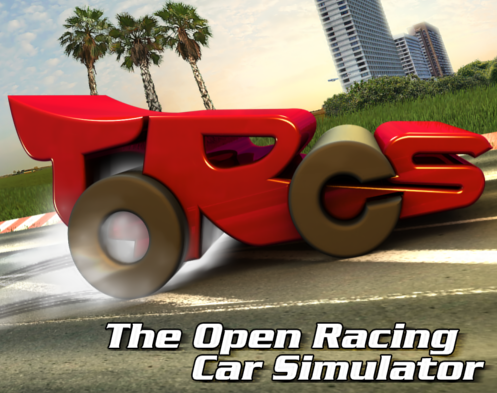
\includegraphics[height=90mm]{images/torcs.png} 
  %\end{center}

  \clearpage
  
  \renewcommand{\labelitemi}{$\bullet$}
  \renewcommand{\labelitemii}{$\circ$}
  \renewcommand{\labelitemiii}{$\diamond$}
  \renewcommand{\labelitemiv}{$\ast$}
  
  
  De part la nature du projet : bibliothèque + interfacement avec le simulateur, l'installation est un peu technique.
  De plus, le fonctionnement sans modification de code est assez limité, il faudra mieux se référer au 
  Manuel du Programmeur pour tirer parti de la bibliothèque.
  
  \section{Procédure d’installation}

  \subsection{Configuration Requise}
  La procédure d'installation doit se dérouler sur un environnement GNU/Linux.
  Le projet est pleinement fonctionnel sur les distributions Archlinux et Ubuntu.
 
  Il vous faudra disposer des drivers graphiques ``hardware'' de votre carte et répondre aux spécifications
  matérielles suivantes :
   \begin{itemize}
    \item 1GHz CPU
    \item 512MB RAM
    \item OpenGL 1.3 compatible graphics card with 64 MB RAM
    \item 2 Go d'espace libre
   \end{itemize}
 
 Au vu de la taille du simulateur TORCS \cite{TORCS} présenté
  dans le cahier des charges \cite{CdC}, il n'a été fourni en même temps que le reste du projet.
 Vous avez donc 2 méthodes pour le récupérer : 
  \subsection{Installer le simulateur : Via la distribution (recommandé sur Ubuntu) }
  
  Si vous êtes sous Ubuntu, TORCS semble avoir quelques problèmes à se lancer après une compilation à la main,
  nous recommandons donc de l'installer directement :
  
    \begin{lstlisting}
sudo apt-get install torcs
    \end{lstlisting}
    
    Vous pouvez alors passer à l'étape 1.4 directement.
   
  \subsection{Installer le simulateur : Via compilation}
  
  Si toutefois, vous souhaitez vous lancer dans la compilation de torcs, voici la marche à suivre : (fonctionne sur 
  Archlinux )
 
  \subsubsection{Liste des paquets pré-requis}
  Voici la liste des paquets que vous aurez besoin afin de compiler le simulateur :
  \begin{multicols}{2}
    \begin{itemize}
    \item bash
    \item gcc (avec g++)
    \item mesa
    \item freeglut
    \item openAL (avec alut)
    \item vorbis
    \item libxi
    \item Xmu
    \item Xrender
    \item Xrandr
    \item libz
    \item libpng
    \end{itemize}
  \end{multicols}
  
  Sur un live CD Ubuntu, la commande suivante est suffisante (en activant tout les dépôts) :
  \begin{lstlisting}
sudo apt-get install g++ mesa-common-dev freeglut3-dev libplib-dev libopenal-dev libalut-dev libvorbis-dev libxi-dev libxmu-dev libxrender-dev libxrandr-dev zlib1g-dev libpng12-dev 
    \end{lstlisting}

  
  L'utilisation de sudo facilite l'installation et ne modifira que les chemins (local est optionnel en fonction de la
  distribution) : 
  \begin{itemize}
    \item /usr/local/share/games/torcs/
    \item /usr/local/lib/torcs/
    \item /usr/local/bin/torcs
  \end{itemize}

  Si vous n'en avez pas l'envie, vous pouvez utiliser un live CD.
  
  \subsubsection{Récupérer le code du simulateur}
  
  
  Il faut maintenant récupérer le code du simulateur 
  
  Pour celà, ouvrez une console et placez vous dans le répertoire Sources/torcs/ et lancer le script 
    \begin{lstlisting}
./getTorcs
    \end{lstlisting}
  Vous devriez alors avoir un dossier /Sources/torcs/torcs-1.3.4/ avec tout les fichiers nécessaires à la compilation.
 
   \subsubsection{Compiler le simulateur}
  
  Toujours dans Sources/torcs/, lancer :
  
  \begin{lstlisting}
./buildTorcs
    \end{lstlisting}
  
  Si vous avez des problèmes lors de cette phase, vous pouvez vous reportez sur l'aide en ligne de TORCS :
  \href{http://torcs.sourceforge.net/index.php?name=Sections&op=viewarticle&artid=30}{FAQ}
  
  \subsection{Compilation du projet}
  
  Voici la liste des paquets que vous aurez besoin afin de compiler le projet :
    
   \begin{multicols}{2}
  \begin{itemize}
    \item make
    \item g++
    \item cmake
    \item sudo
    \item boost (system, serialization, filesystem)
    \item libplib
  \end{itemize}
    \end{multicols}

  Sur ubuntu : 
    \begin{lstlisting}
sudo apt-get install g++ cmake libboost-dev libboost-system-dev libboost-serialization-dev libboost-filesystem-dev libplib-dev
    \end{lstlisting}
    
    Vous êtes alors prêt à lancer la dernière compilation.
    
    Pour celà, il faut se rendre dans le dossier Sources/ et lancer
    \begin{lstlisting}
./makeDriver
    \end{lstlisting}
    
  \section{Désinstallation}
  
 
  \section{Paramètres de fonctionnement}


  
  
  
  \section{Fonctionnalités et interactions utilisateur}

  
  

\addcontentsline{toc}{section}{Références}
\bibliographystyle{../dependance/apalike}
\bibliography{../dependance/biblio}

\end{document}



